\chapter{Módulo 1: Preparación}

Iniciaremos con la placa np07

\begin{figure}[h]
	\centering
	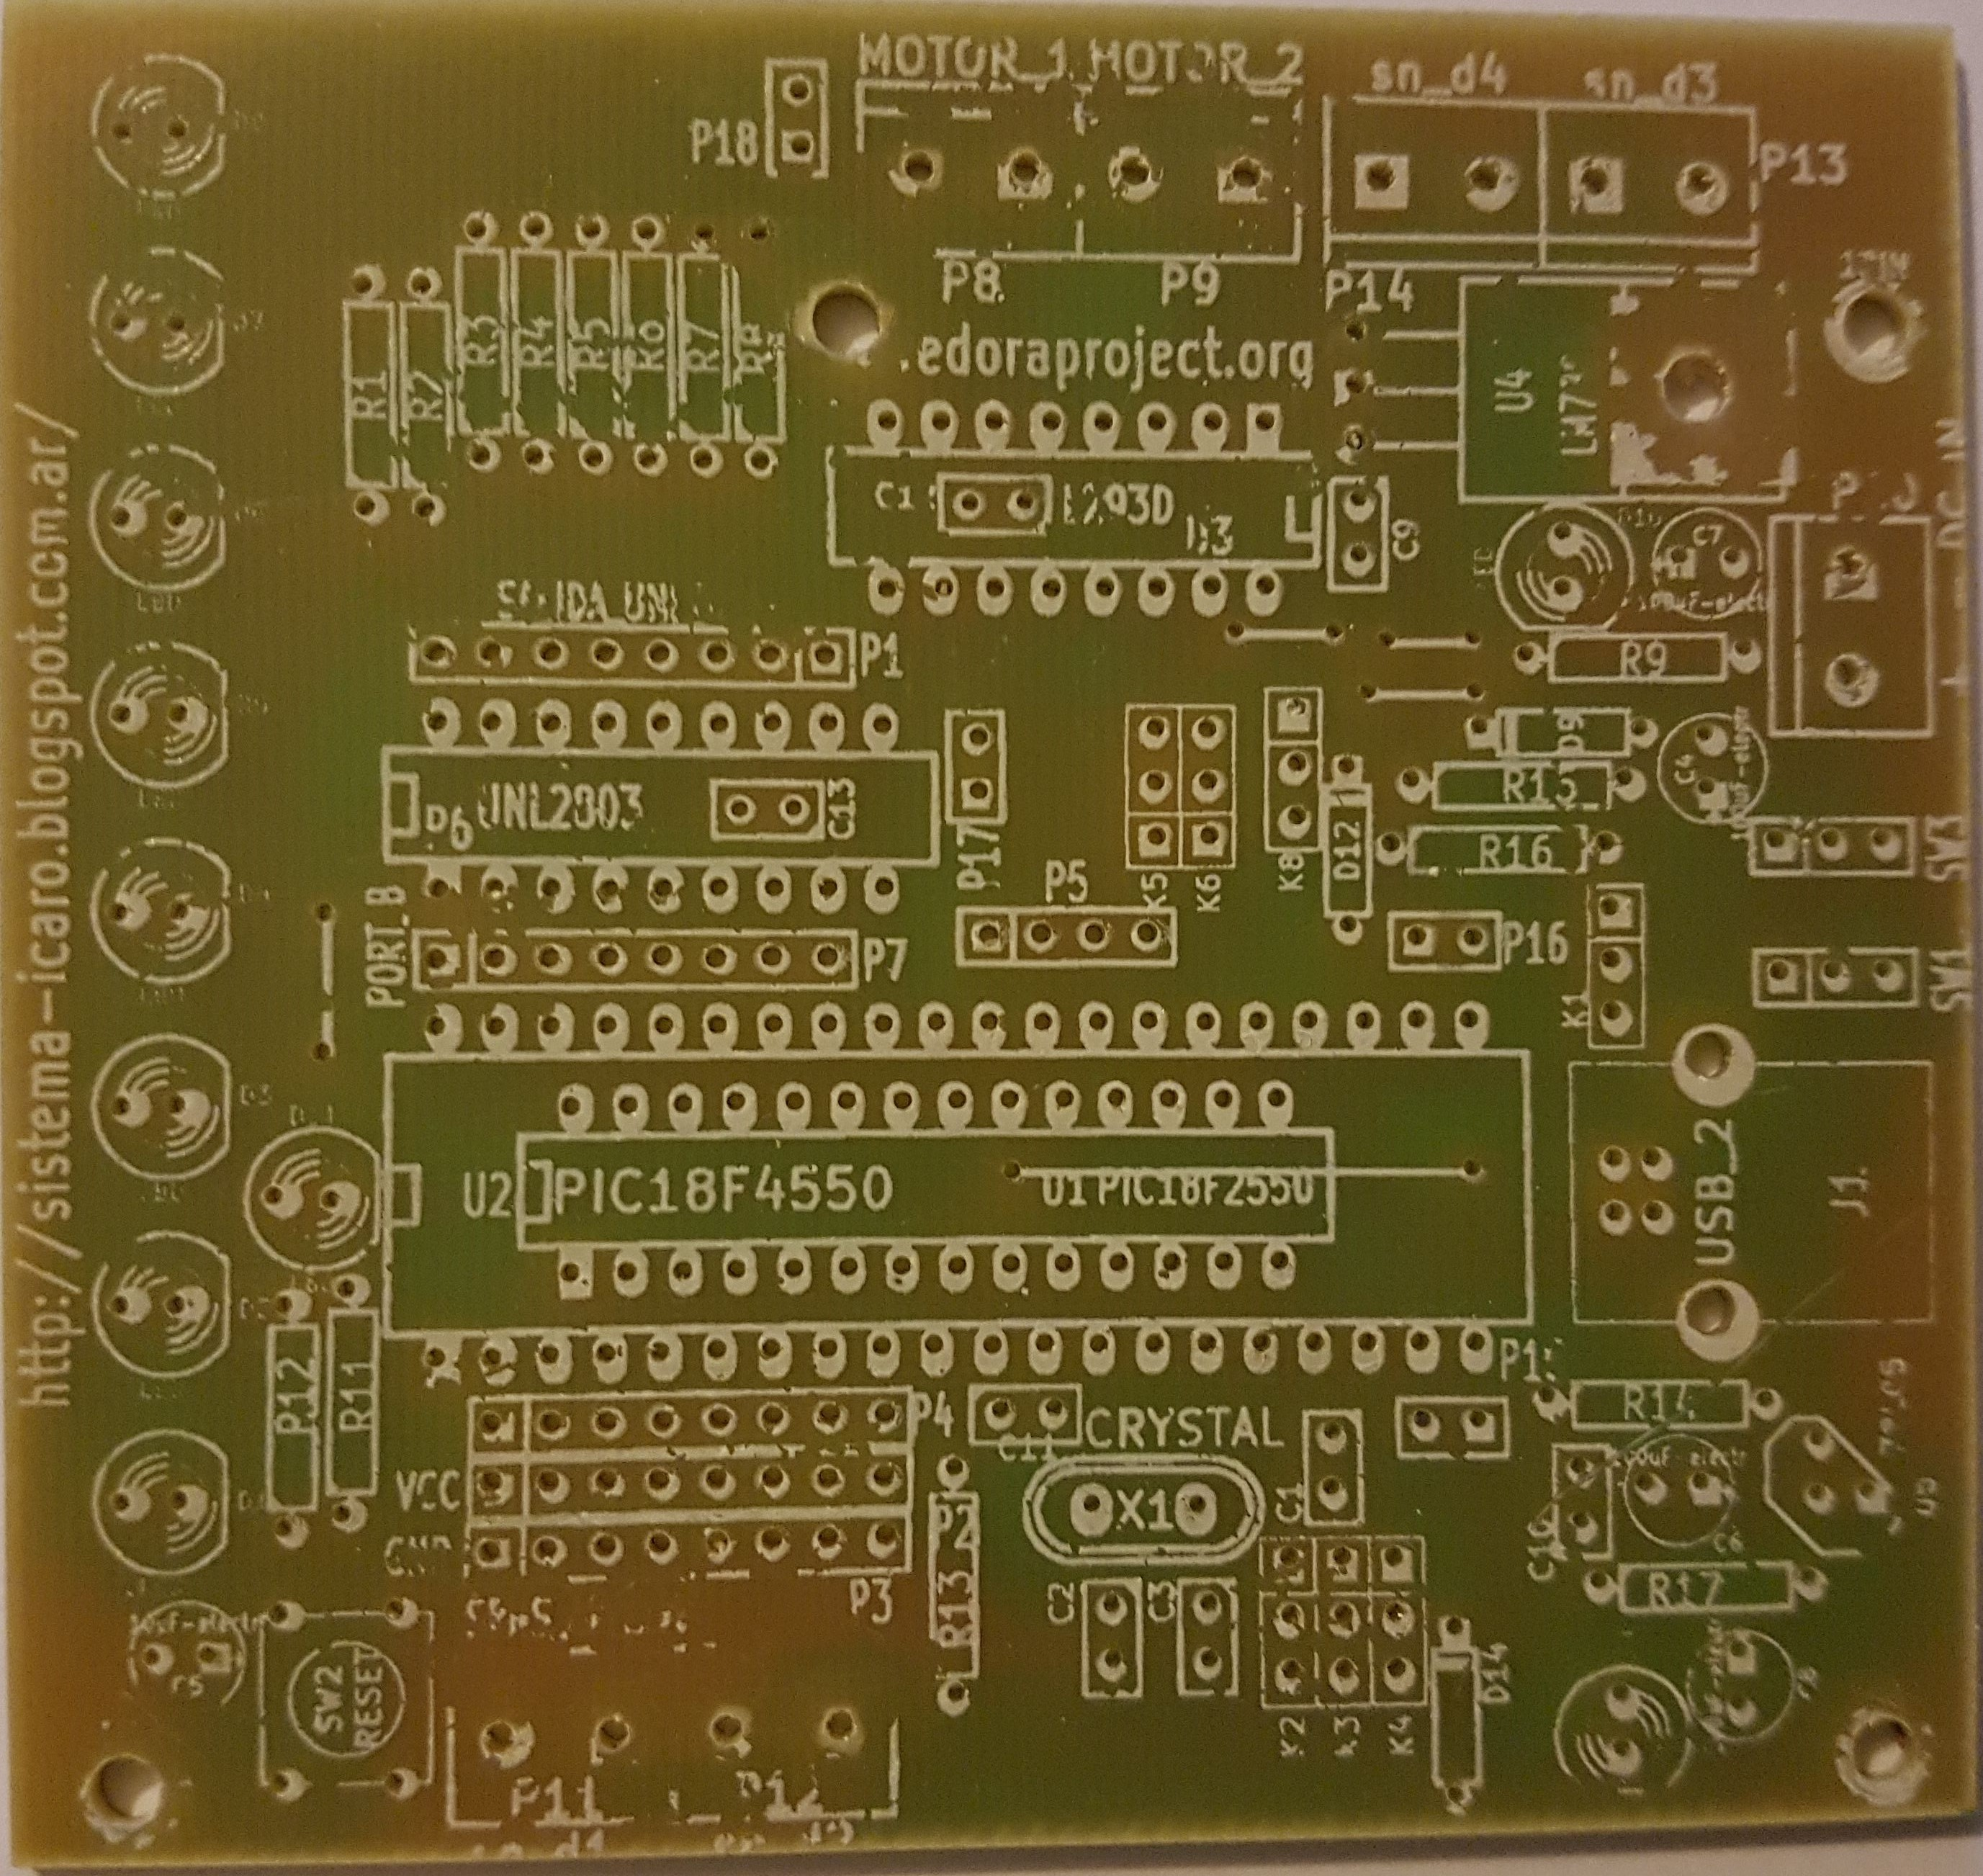
\includegraphics[width=0.8\linewidth]{Modulo_1/M1_0}
	\caption{Módulo 1 - Placa np07}
	\label{fig:M1_0}
\end{figure}

\newpage

\section{Paso 1:}

Instalar los 5 puentes de la placa. Para el puente que quedará bajo el Microcontrolador se requiere un pedazo de cable. Lo más común es cable UTP de redes, pelado. La cubierta del cable se derretirá de todas formas al soldarlo. Los otros puentes se pueden hacer usando más de este tipo de cable o se puede usar patitas de resistencias.

\begin{figure}[h]
	\centering
	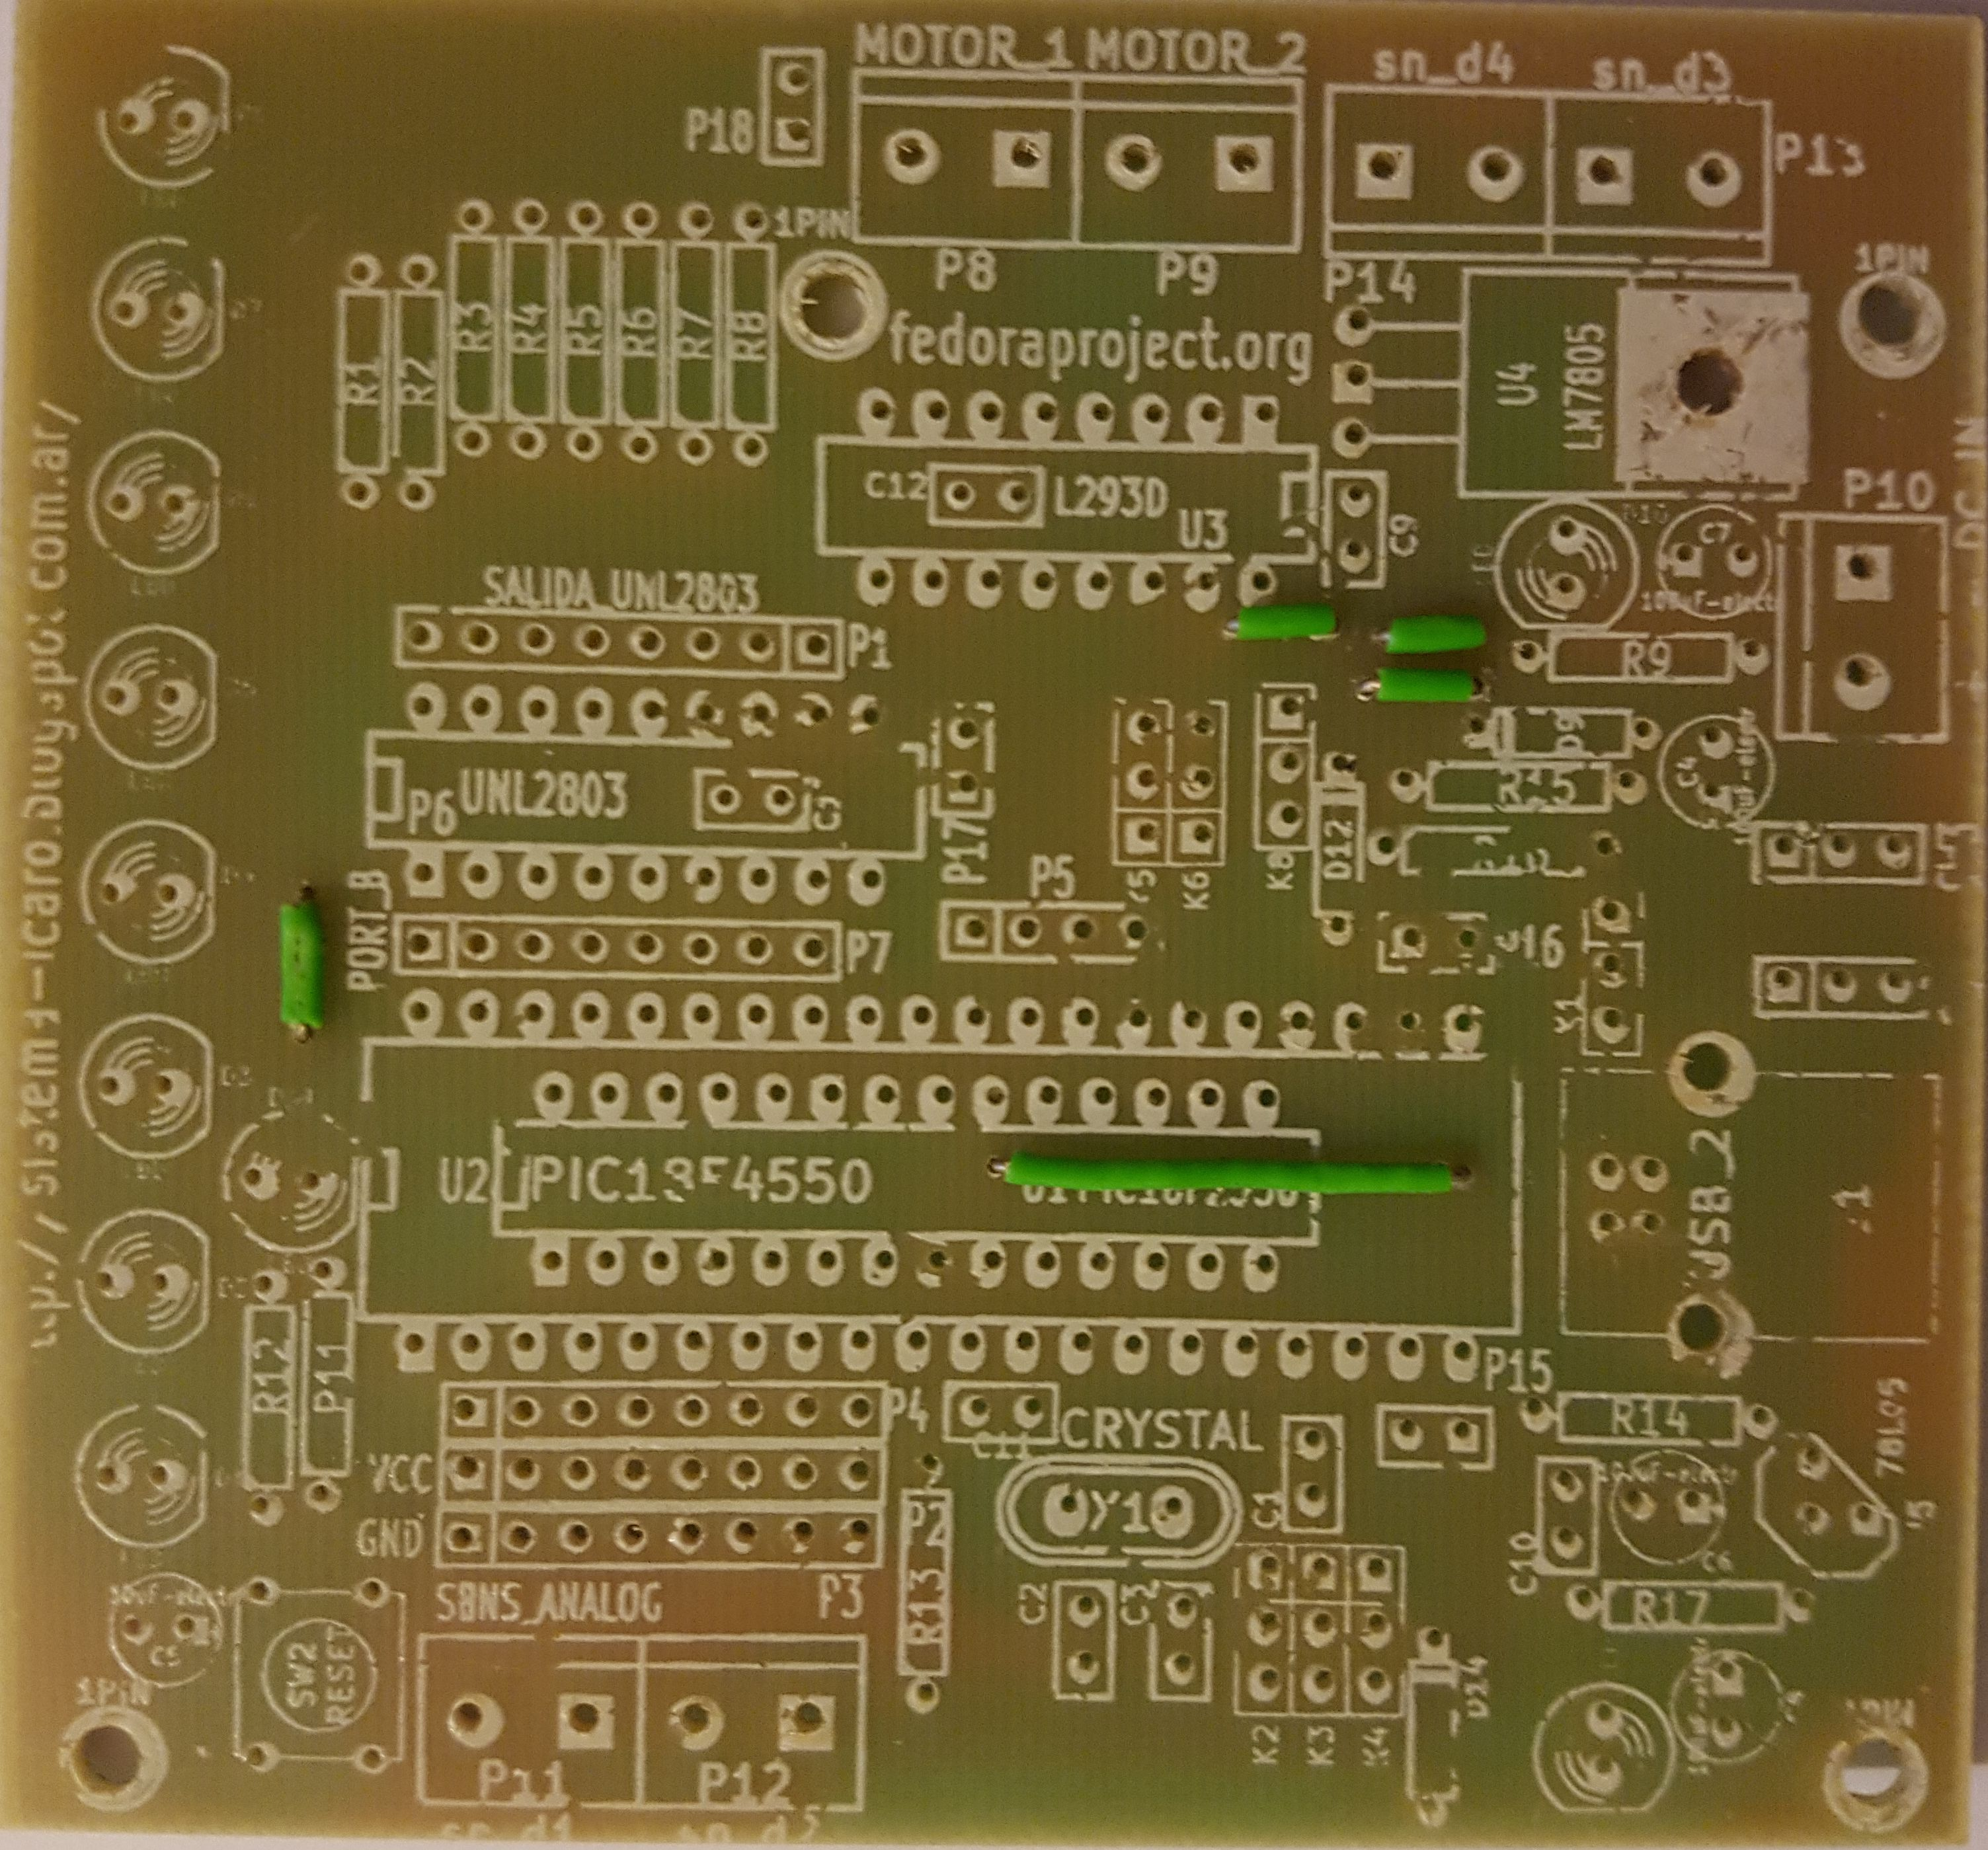
\includegraphics[width=0.8\linewidth]{Modulo_1/M1_1}
	\caption{Módulo 1 - Paso 1}
	\label{fig:M1_1}
\end{figure}

\newpage

\section{Paso 2:}

Instalar todos los diodos. D9, D12 y D14

\begin{figure}[h]
	\centering
	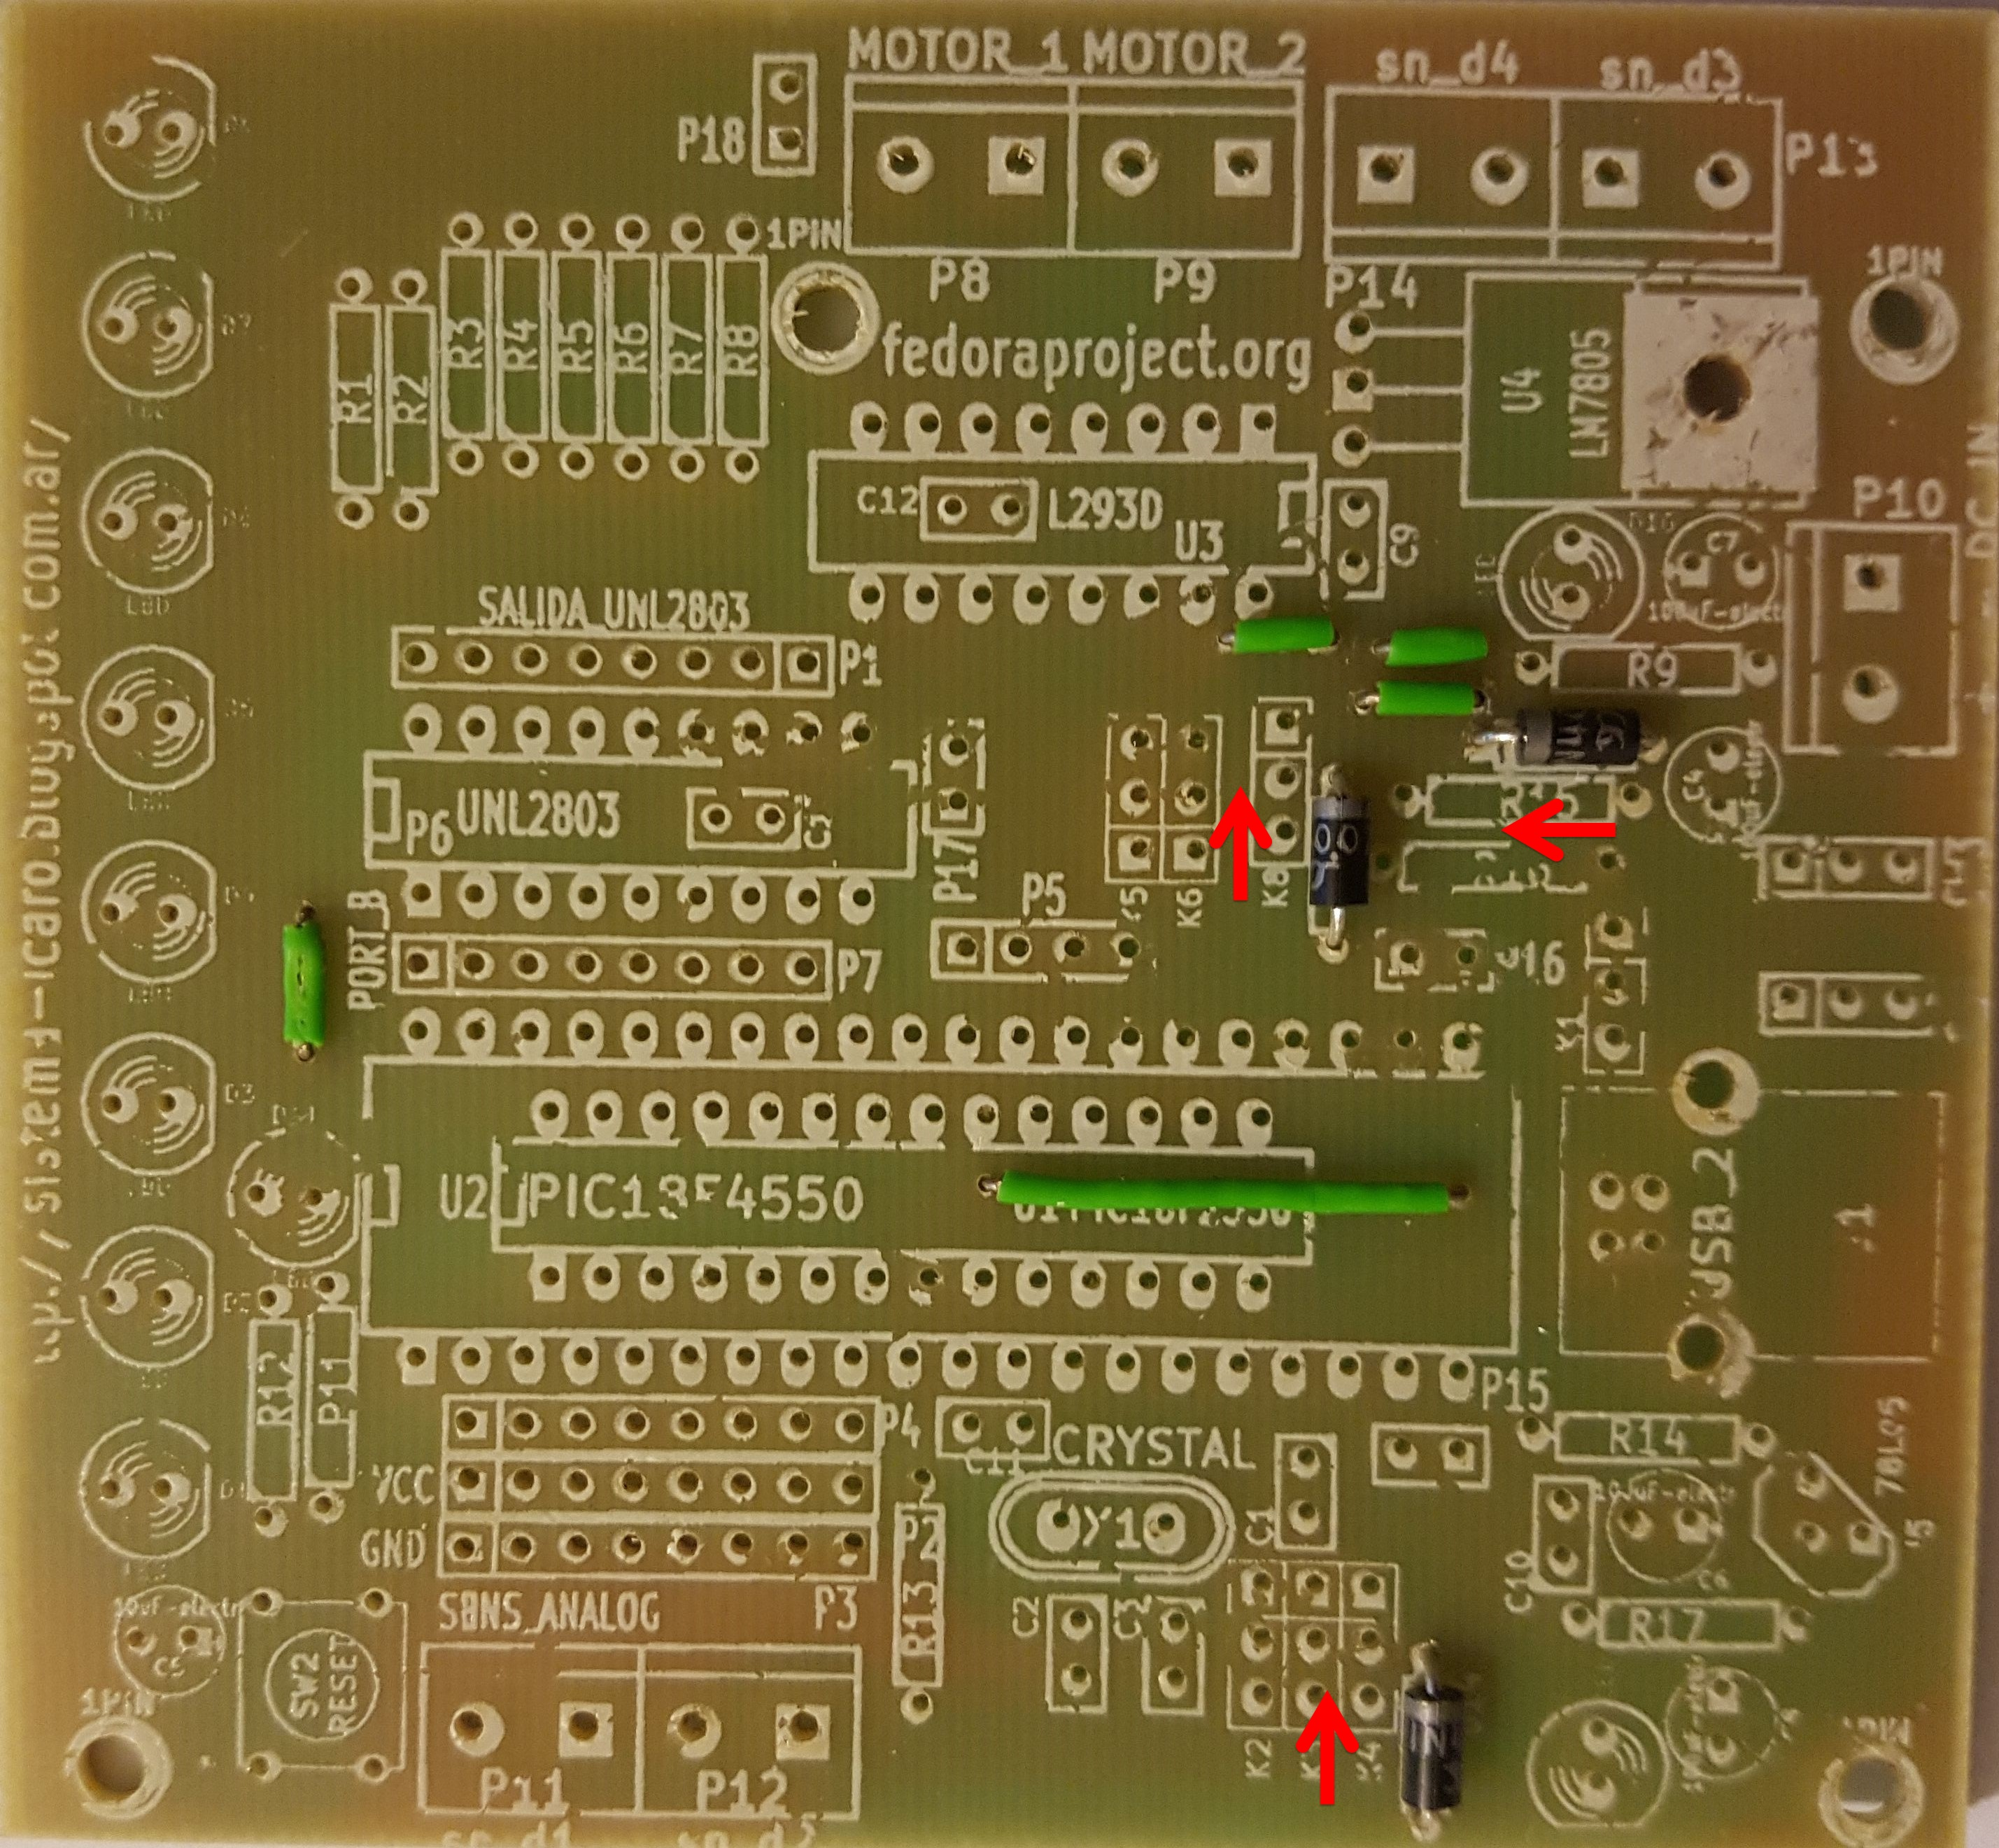
\includegraphics[width=0.8\linewidth]{Modulo_1/M1_2}
	\caption{Módulo 1 - Paso 2}
	\label{fig:M1_2}
\end{figure}

\newpage

\section{Paso 3:}

Instalar las resistencias de 470 Ohm. R9, R12 y R17

\begin{figure}[h]
	\centering
	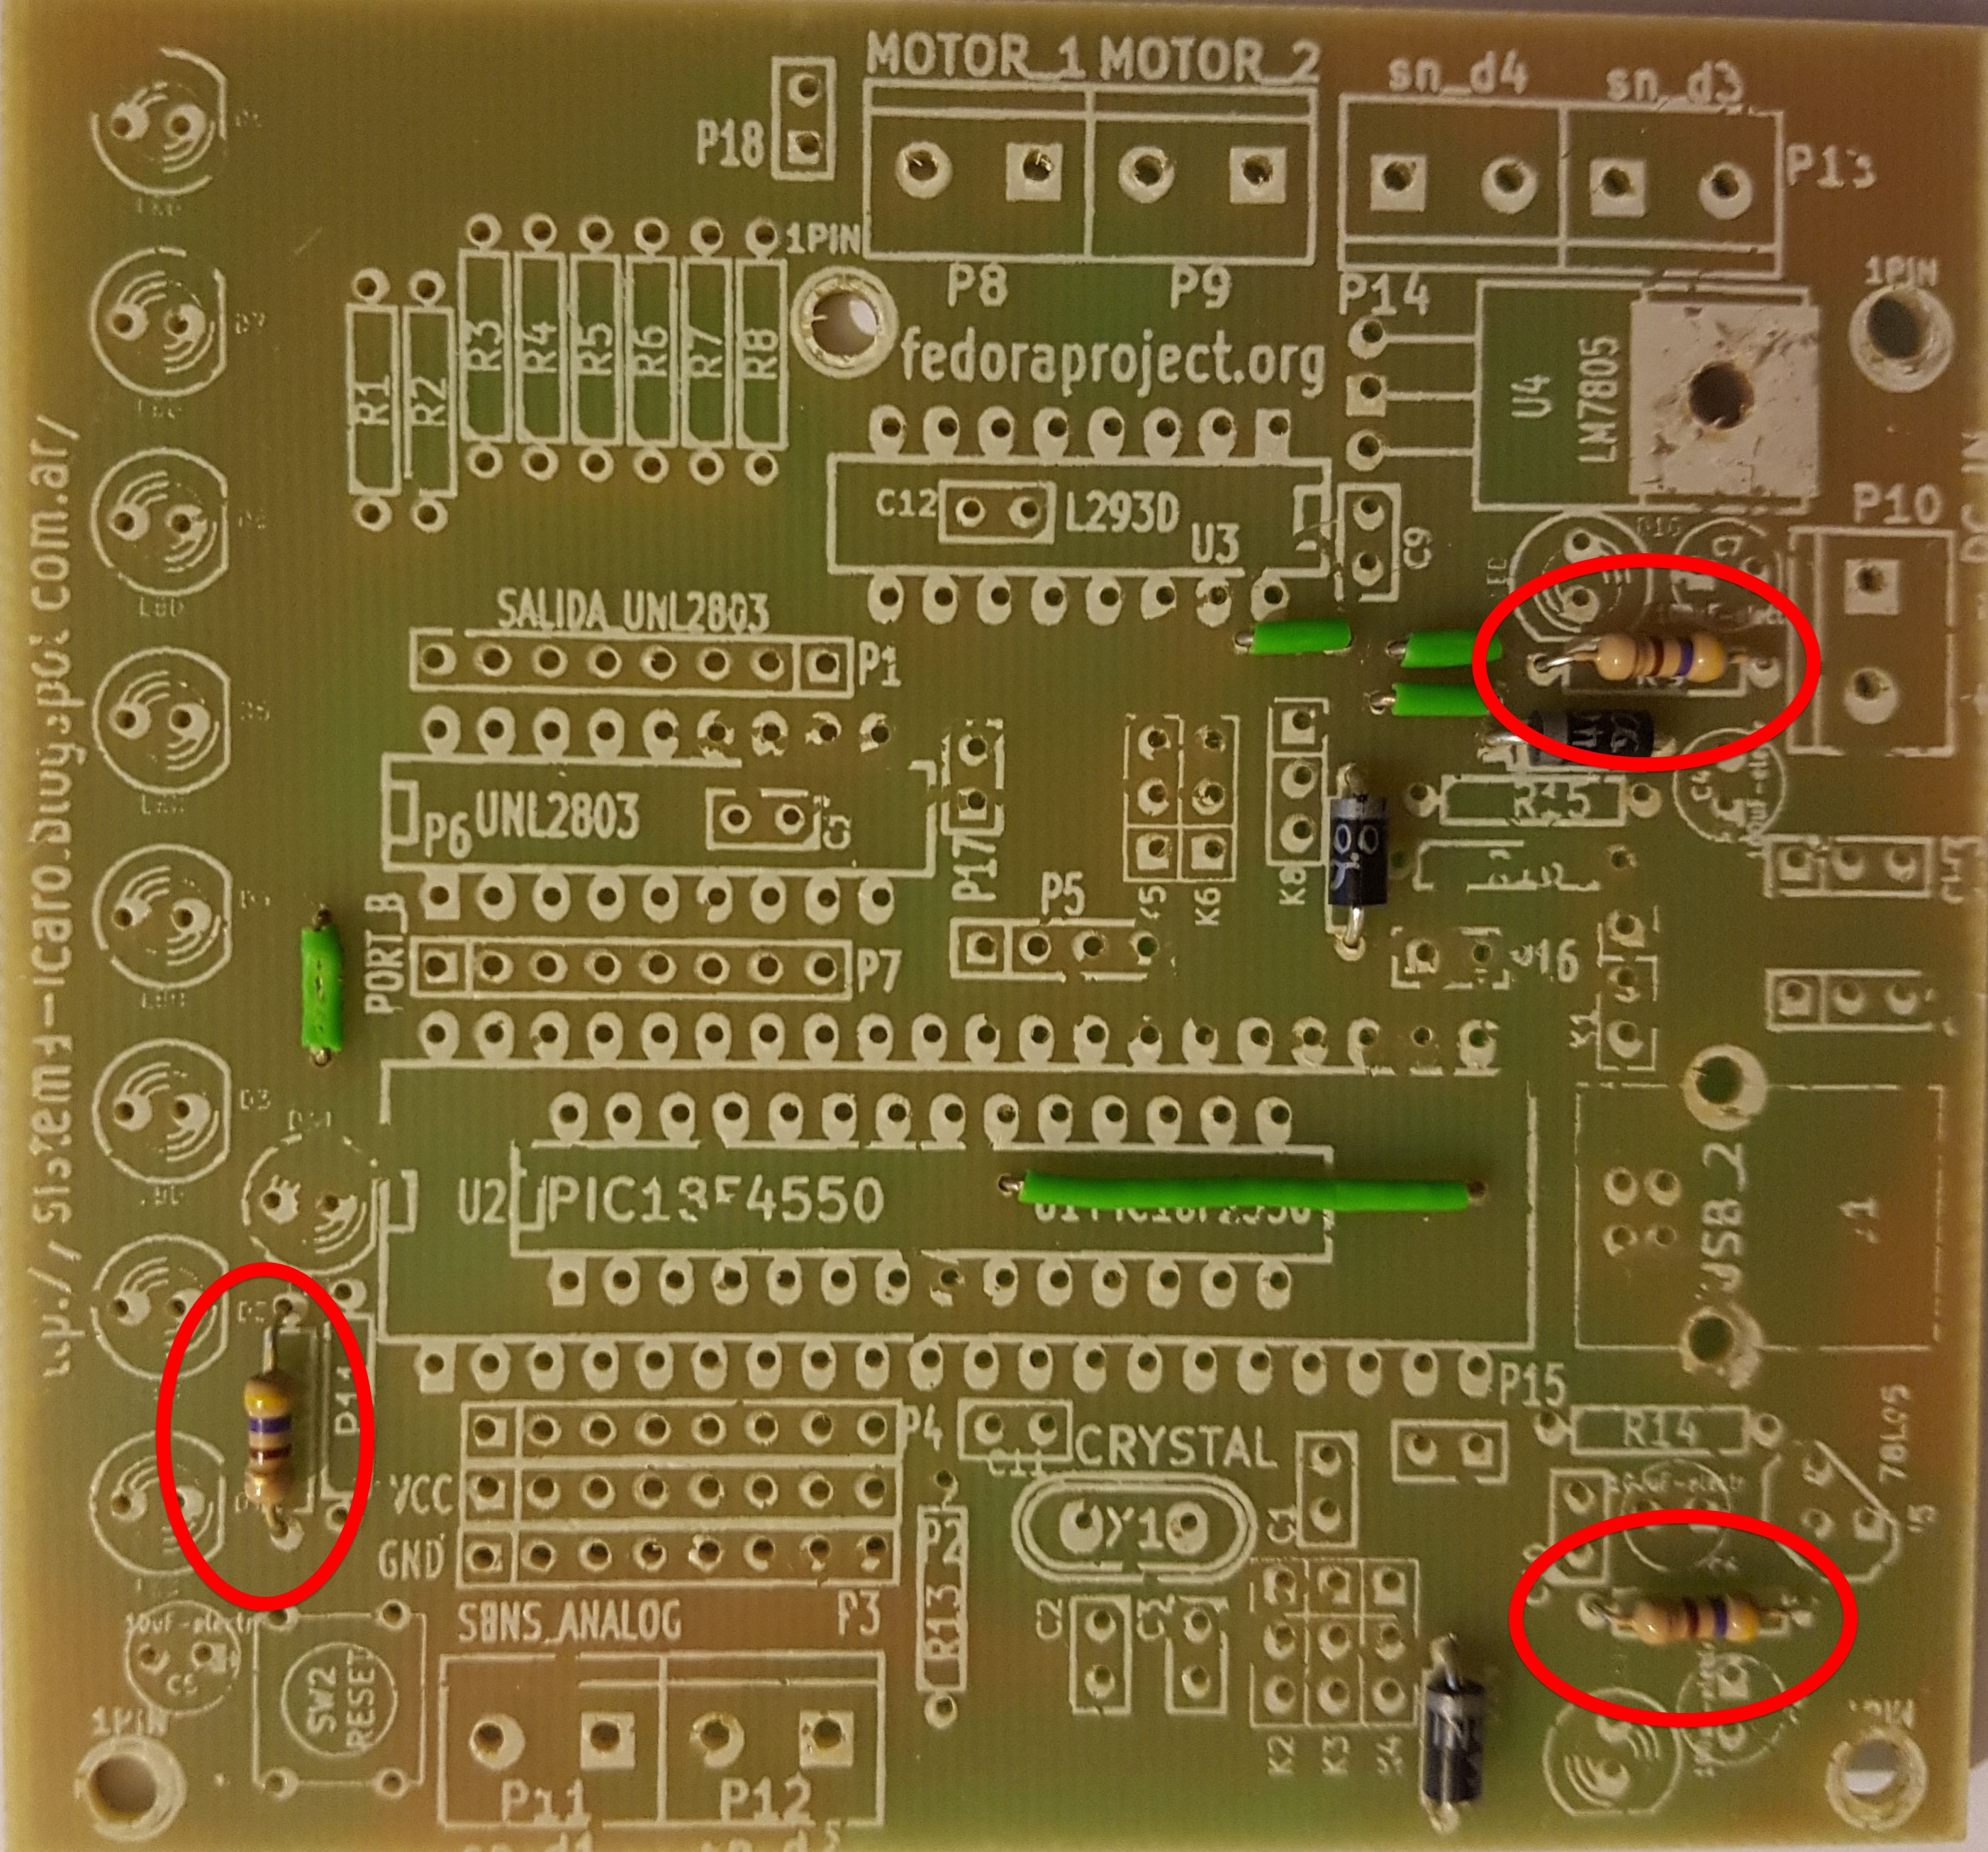
\includegraphics[width=0.8\linewidth]{Modulo_1/M1_3}
	\caption{Módulo 1 - Paso 3}
	\label{fig:M1_3}
\end{figure}

\newpage

\section{Paso 4:}

Instalar las resistencias de 10K Ohm. R11, R13, R14, R15 y R16

\begin{figure}[h]
	\centering
	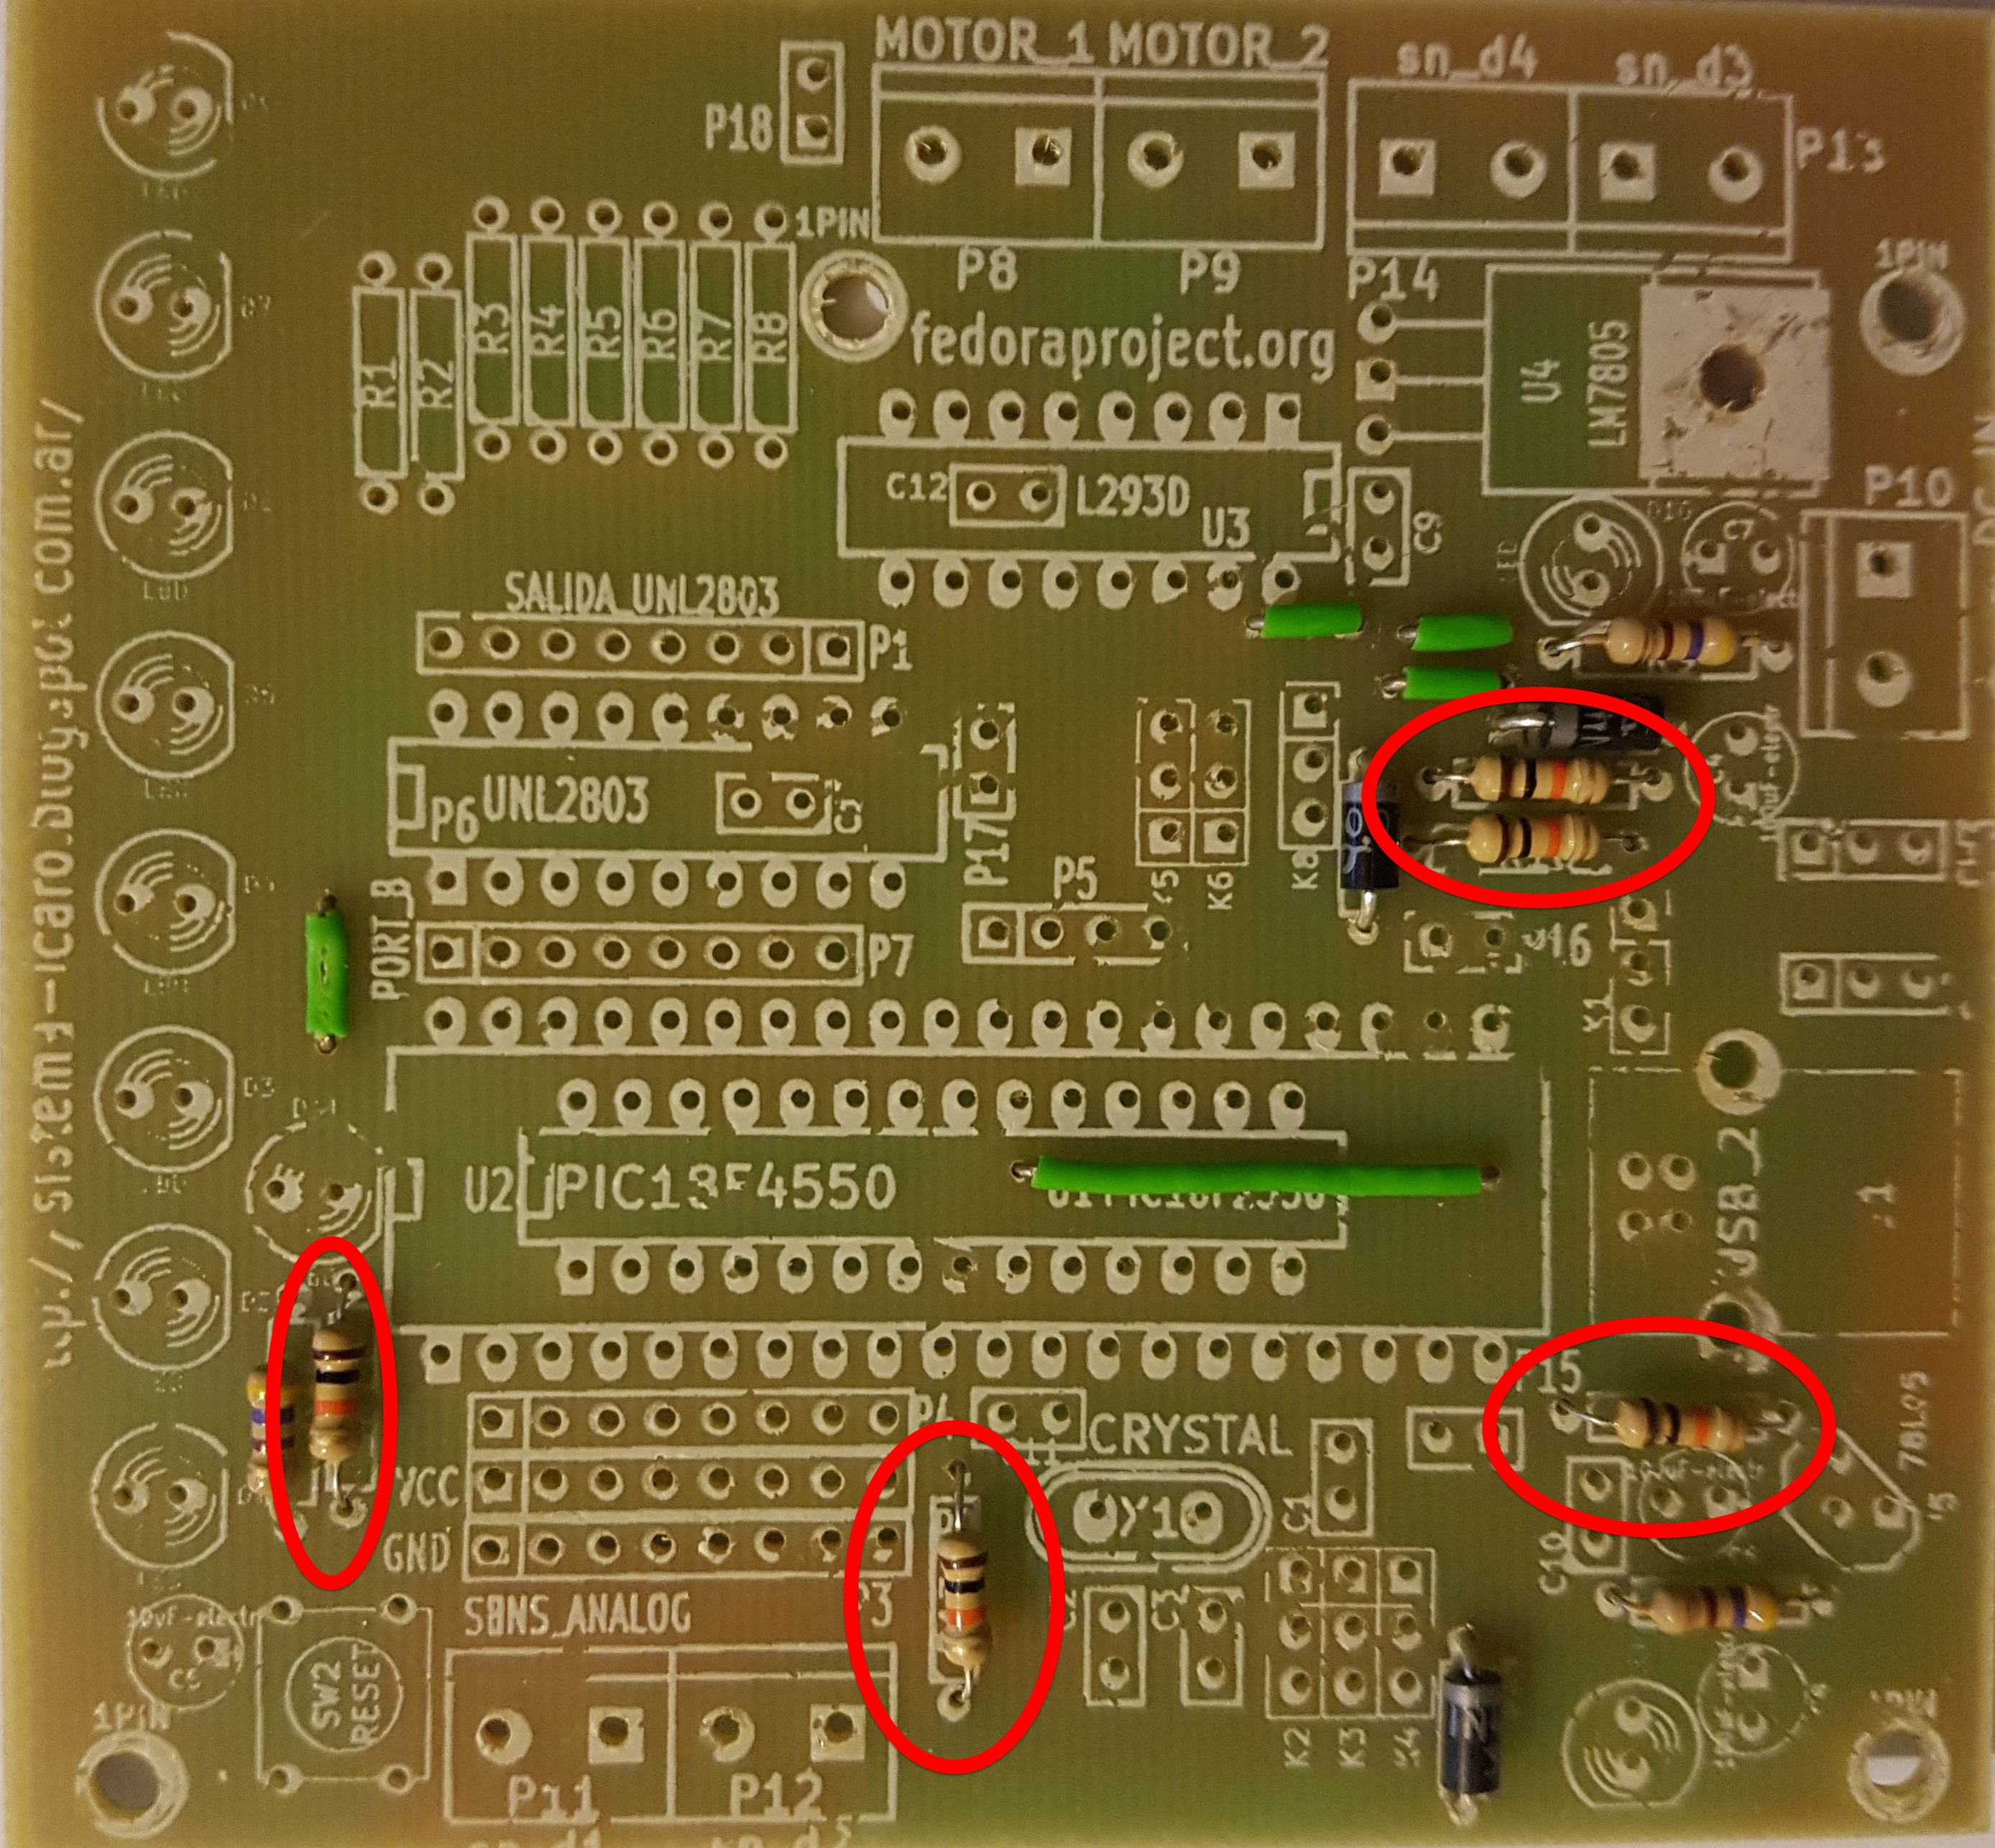
\includegraphics[width=0.8\linewidth]{Modulo_1/M1_4}
	\caption{Módulo 1 - Paso 4}
	\label{fig:M1_4}
\end{figure}

